%\chapterauthor{Author Name}{Author Affiliation}
%\chapterauthor{Second Author}{Second Author Affiliation}
\chapter{Files Management}

File management is a big portion of OS functionality. In Linux, each device (such as a printer) is treated and managed as a file, and Linux uses a tree hierarchy to manage devices and files. This chapter introduces the filesystem hierarchy and commonly used file management commands.

\section{Filesystem Hierarchy Standard} \label{ch4sec:hierarchy}

The root directory is denoted by \verb|/|. All sub directories or files can be located by its full path, which looks like the following
\begin{lstlisting}
/<subdirectory>/<subsubdirectory>/.../<directoryname>
/<subdirectory>/<subsubdirectory>/.../<filename>
\end{lstlisting}
where the first \verb|/| in each row represents the root directory, and sequential \verb|/| represents entering a subdirectory.

Upon Linux installation, a file hierarchy is by default created under the root directory. A user can create new files under this hierarchy framework, but should not change the framework itself. The hierarchy is given in Fig. \ref{ch4fig:hierarchy}. Notice that ``\verb|/|'' in the figure, as introduced, stands for the root directory, and ``\verb|root|'' in the figure is a subdirectory under \verb|/| whose directory name is ``root'' and it is used store root user related documents. They are two different directories.

\begin{figure}
	\centering
	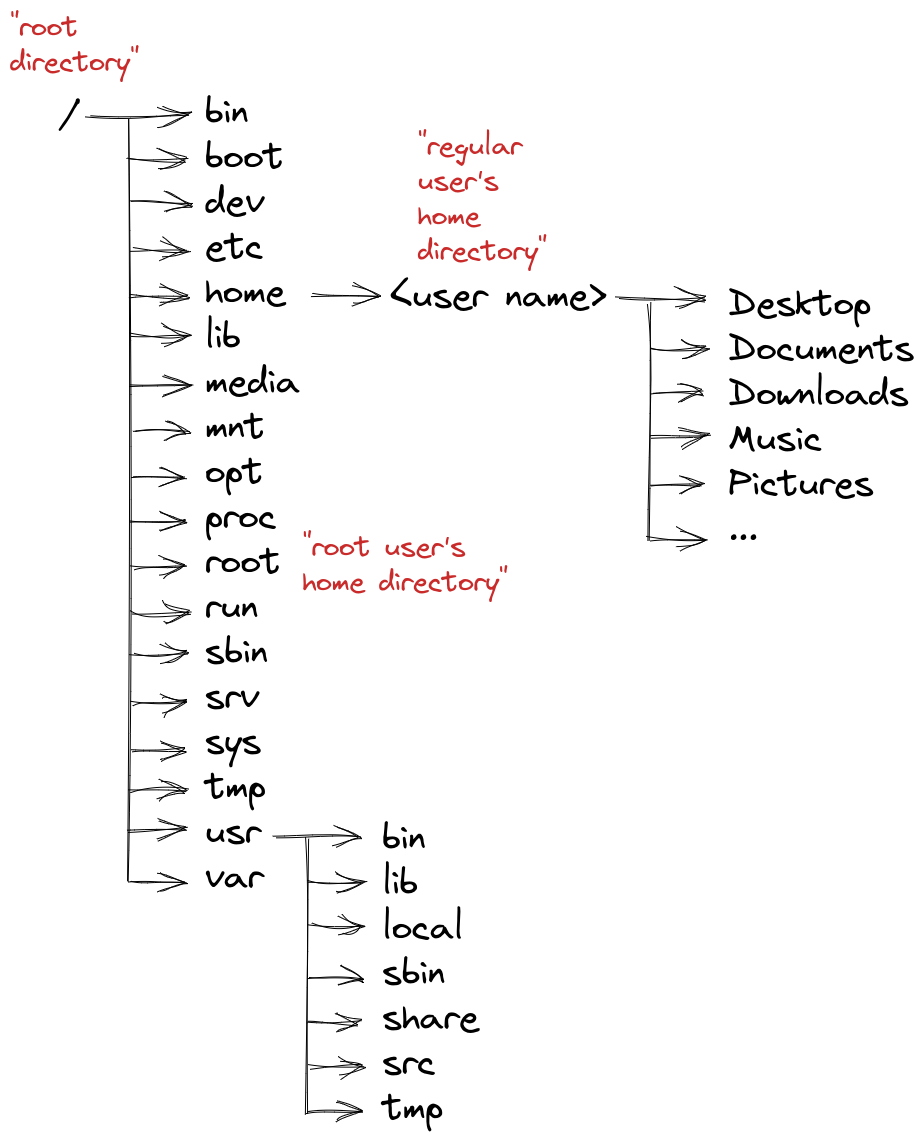
\includegraphics[width=250pt]{chapters/chapter4/figures/linux_file_hierarchy.png}
	\caption{Linux file system hierarchy.} \label{ch4fig:hierarchy}
\end{figure}

A (regular) user's home directory is often located at \verb|/home/<user name>|. When logging in as a regular user, his home directory is shorten by the tilde \verb|~| for convenience. Hence, for example \verb|ls ~| will list down the files and directories under his home directory.

As can be seen from Fig. \ref{ch4fig:hierarchy}, the hierarchy contains quite a few pre-determined subdirectories, each has some unique purpose. For convenience of illustration, these subdirectories are categorized by functionalities and depressibilities given in Fig. \ref{ch4fig:directorycate}. Notice that this categorization is rough and may not reflect the truth for all applications. For example, the commonly used command \verb|ls| may appear under \verb|/bin| or \verb|/usr/bin| depending on the Linux distributions.

\begin{figure}
	\centering
	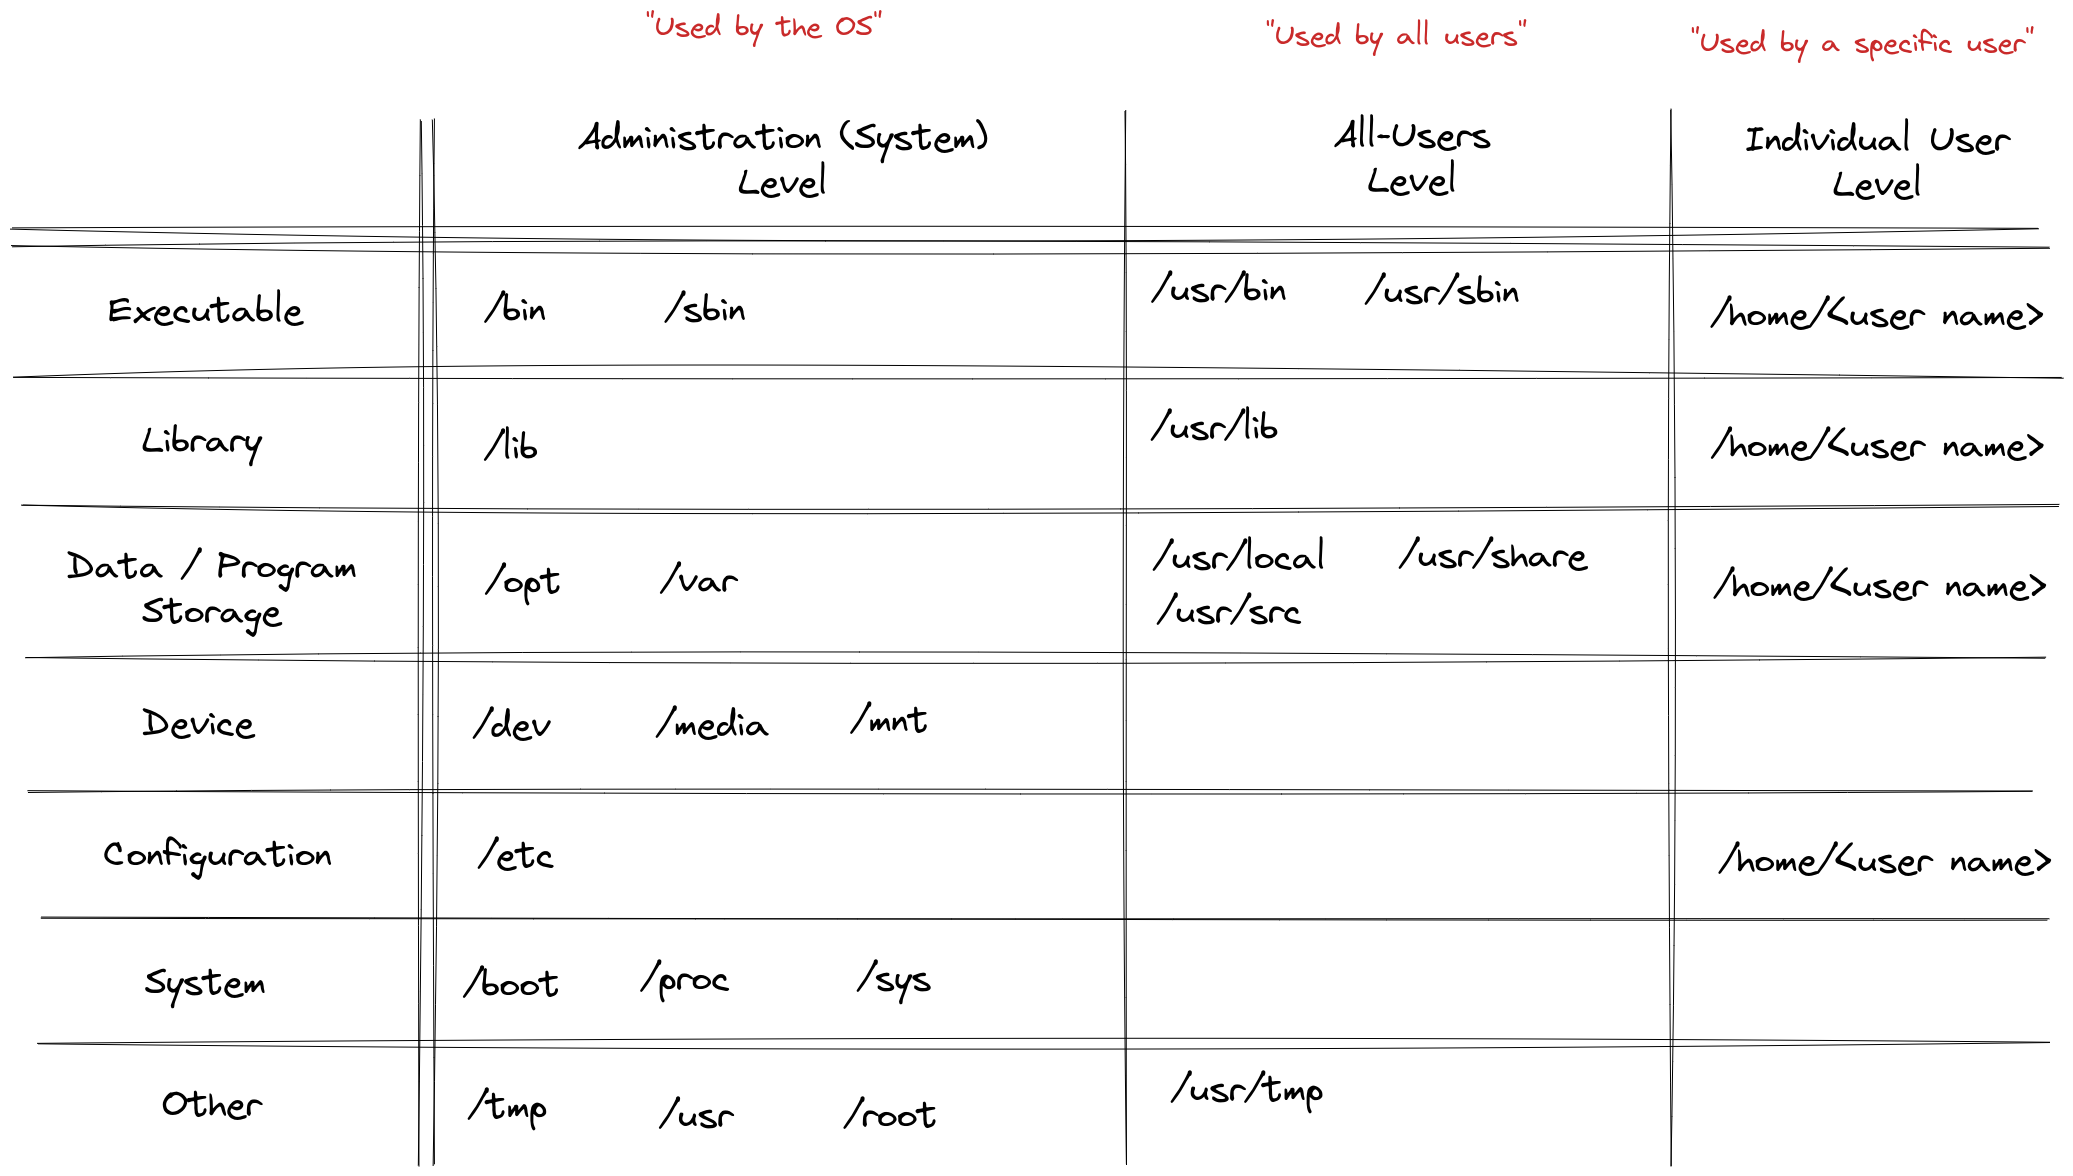
\includegraphics[width=350pt]{chapters/chapter4/figures/linux_directory_cate.png}
	\caption{A rough categorization of commonly used directories in Linux file hierarchy standard.} \label{ch4fig:directorycate}
\end{figure}

A brief introduction to the directories are summarized in Table \ref{ch4tab:hierarchyintro}.

\begin{table}
  \centering \caption{Introduction to commonly used directories in Linux file hierarchy standard.}\label{ch4tab:hierarchyintro}
  \begin{tabularx}{\textwidth}{lX}
    \hline
    Directory & Description \\ \hline
    \verb|/bin|, \verb|/sbin| & Executables used by the OS, the administrator, and the regular users. \\ \hdashline
    \verb|/lib| & Libraries to support \verb|/bin| and \verb|/sbin|. \\ \hdashline
    \verb|/usr/bin|, \verb|/usr/sbin| & Executables used by the administrator and the regular users. \\ \hdashline
    \verb|/usr/lib| & Libraries to support \verb|/usr/bin| and \verb|/usr/sbin|. \\ \hdashline
    \verb|/opt| & Application software installed by OS and administrator for all users. \\ \hdashline
    \verb|/var| & Directories of data used by applications. \\ \hdashline
    \verb|/usr/local| & Application software installed by administrator for all users. \\ \hdashline
    \verb|/usr/share| & Architecture-independent sharable text files for applications. \\ \hdashline
    \verb|/usr/src| & Source files or packages managed by software manager. \\ \hdashline
    \verb|/dev| & Files representation of devices, such as CPU, RAM, hard disks. \\ \hdashline
    \verb|/media| & System mounts of removable media. \\ \hdashline
    \verb|/mnt| & Manual mounts of devices. \\ \hdashline
    \verb|/etc| & Configuration files for OS, users, and applications. \\ \hdashline
    \verb|/boot| & Linux bootable kernel and initial setups. \\ \hdashline
    \verb|/proc| & System resources information. \\ \hdashline
    \verb|/sys| & Linux kernel information, including a mirror of the kernel data structure. \\ \hdashline
    \verb|/tmp|, \verb|usr/tmp| & Temporary files. \\ \hdashline
    \verb|/root| & Root user's home directory. \\ \hdashline
    \verb|/home/<user name>| & A regular user's home directory, containing executables, configurations and files specifically belong to this user. \\
    \hline
  \end{tabularx}
\end{table}

Linux file hierarchy standard differs from MS-DOS and Windows in several ways. Firstly, Linux stores all files (regardless of their physical location) under root directory, while Windows uses drive letters such as \verb|C:\|, \verb|D:\| to distinguish different hard drives. Secondly, Linux uses slash (\verb|/|) to separate directory names, e.g. \verb|/home/username| while Windows uses back slash (\verb|\|), e.g. \verb|C:\Users\username|. Lastly, Linux uses ``magic numbers'' to tell file types and permissions and ownership to tell whether a file is executable, while Windows (almost always) uses suffixes to tell file types and distinguish executables. Distinguishing file types using magic numbers can be more reliable than using suffixes, though a bit less intuitive.

Magic numbers of a file refer to the first few bytes of a file that are unique to a particular file type, for example, PNG file is hex \verb|89 50 4e 47|. Linux compare the magic numbers of a file with an internal database to decide the file types and features.

\section{Commonly Used File Management Commands} \label{ch4sec:filemanagement}

Some of the most widely used file management commands are summarized in Table \ref{ch4tab:commonfilecommands}. Notice that \verb|chmod| and \verb|chown| are administration related commands that change the accessibility of a directory or a file, and will be introduced in a later sections together with the Linux permission system. The rest commands are categorized and introduced in the following subsections.

\begin{table}
  \centering \caption{Commonly used commands to navigate in the Linux file system.}\label{ch4tab:commonfilecommands}
  \begin{tabularx}{\textwidth}{lX}
    \hline
    Command & Description \\ \hline
    \verb|pwd| & Print working directory. \\ \hdashline
    \verb|ls| & List the subdirectories and files (and their detail information) in a given directory. \\ \hdashline
    \verb|touch| & Create an empty file. \\ \hdashline
    \verb|mkdir| & Create an empty subdirectory. \\ \hdashline
    \verb|mv| & Cut-ant-paste a directory or a file; change name of a directory or a file. \\ \hdashline
    \verb|cp| & Copy-and-paste a directory or a file. \\ \hdashline
    \verb|rm|, \verb|rmdir| & Remove a directory or a file (not to Trash, but just gone). \\ \hdashline
    \verb|chmod| & Change permission. \\ \hdashline
    \verb|chown| & Change ownership. \\
    \hline
  \end{tabularx}
\end{table}

\subsection{Print Working Directory}

As introduced earlier in Chapter \ref{ch2} Table \ref{ch2tab:shellenvironmentvars}, \verb|HOME|, \verb|PWD| and \verb|OLDPWD| are three default environmental variables used to store the home directory, the current directory and the previous directory of the shell, respectively. Therefore, to print the current working directory in the console, use command \verb|echo $PWD|. Alternatively, just use \verb|pwd| which has the safe effect.

\subsection{List Information about the Files}

As one of the most frequently used commands, \verb|ls| lists down information about the files in the current directory, and by default sort the entries alphabetically. 










